\documentclass[10pt,twocolumn,letterpaper]{article}

\usepackage{cvpr}
\usepackage{times}
\usepackage{epsfig}
\usepackage{graphicx}
\usepackage{amsmath}
\usepackage{amssymb}

% Include other packages here, before hyperref.

% If you comment hyperref and then uncomment it, you should delete
% egpaper.aux before re-running latex.  (Or just hit 'q' on the first latex
% run, let it finish, and you should be clear).
\usepackage[breaklinks=true,bookmarks=false]{hyperref}

\cvprfinalcopy % *** Uncomment this line for the final submission

\def\cvprPaperID{****} % *** Enter the CVPR Paper ID here
\def\httilde{\mbox{\tt\raisebox{-.5ex}{\symbol{126}}}}

% Pages are numbered in submission mode, and unnumbered in camera-ready
%\ifcvprfinal\pagestyle{empty}\fi
\setcounter{page}{1}
\begin{document}

%%%%%%%%% TITLE
\title{Project Report\\
TellGAN: Motion Prediction and Video Generation From Natural Text}

\author{Gunhee Lee, Jacob Morton\\
20172811, 20172327\\
Computer Science and Engineering, POSTECH\\
{\tt\small victorleee@postech.ac.kr}
}


\maketitle
%\thispagestyle{empty}


%%%%%%%%% BODY TEXT
\section{Abstract}

 We propose a Tell Generative Adversarial Network (TellGAN) which, given an initial starting frame with landmarks and text that describes an action, will generate plausible video frames of the given target performing the action. We call it TellGAN, because we tell the target what to do. Our method is a generic end-to-end approach that predicts motion and generates video frames. We divide the task into two parts, landmark trajectory prediction from a given word and generating a video frames from the predicted landmarks and initial target position. We also propose a novel use of an LSTM to predict motion over a various number of frames, to model motions at different speeds. We chose mouth motion prediction for a given word as an application for our model. Although this application is related to lip reading (video-to-text), a well researched area, it appears that text-to-video face motion has not been approached directly before.  Among the several datasets used for lip reading, we used the GRID Corpus\footnote{http://spandh.dcs.shef.ac.uk/gridcorpus/}.
 
%------------------------------------------------------------------------
\section{Introduction}
 Motion Prediction is a well researched area with several existing approaches that predict landmarks using RNN and LSTM networks. Although these networks are able to predict motions given an action, they currently can only learn and predict actions at a constant rate of change, basically learning an average representation. This is a problem in real life, when actions are performed at different rates by different individuals and times. Our model can learn and predict motions performed at various speeds. To our knowledge this problem hasn't been tackled yet. We are able to train an LSTM motion predictor to learn an 'oversampled' representation of the action learned at a higher rate than available from the ground truth. We use a weak loss for predictions with missing ground truths and rely on the dataset to provide various sequence length actions to correctly train the network. We chose a lib-reading dataset to provide a large number of actions with varying rates of speed to train and test our model on text-driven animation.

 Text-Driven animation is not a new topic, but the current approaches use text-to-speech generators to drive animation and are not typically generic. There has been some recent independent techniques developed concurrently with ours that use Generative Adversarial Networks (GAN) for generating video frames, but again use audio as a driving factor. Text-to-speech techniques offer several advantages as there are plenty of previous works and is an easier task to map continuous wave forms rather than discrete words to the motions of the mouth during speech. Our proposed method will skip the text-to-speech generation by training a GAN and an LSTM with the aid of lip-reading techniques. Visual only lip reading is a heavily research topic and is essentially a video-to-text and action classification problem. Our proposed approach is the inverse to lip reading, a Text-to-Video and action generation problem. Generating compelling speech motions from words is a challenging problem. Humans are good at recognizing fine facial movements and can intemperate words from mouth motions. Also most motion prediction techniques don't demonstrate predictions of the fine motions required to model speech.

 Generative adversarial networks have improved in recent years. There also has been research which relates generative adversarial network and natural language processing. Text-to-image generation is one of the most obvious examples of it. Using a GAN to Generate video or images from changing landmarks is currently an active area of research. We use a UNet architecture that takes as input an initial frame and desired landmark positions to change the image to the desired state. The results are of a high degree of realism, where the line between a fake image and real image is blurred.
 
 Our 2-step frame prediction offers more flexibility than previous approaches for the length of action being learned and predicted in addition to generating photo-realistic results. Compared with the normal image generation model, our model receives the input image. The contemporary state of the art network called AttentionGAN (Tao Xu et al.) can only change the image as a whole to meet the sentence direction, which is not desirable. For example, the minor changes that occur between frames would result in a completely different image. Our model would make the image more controllable than the previous approach. Also our model has a temporal component, as we propose generating a series of images that correspond spoken motions derived from the given input to make a video sequence. This has several challenges, among which are maintaining temporal coherency and preventing errors cascading through future generated frames. Previous work on text-to-video using GAN exists\footnote{Video Generation From Text (Li, 2017)}. We will not use this method, as we will not have an end frame nor do we wish to use simultaneous generation of frame sequences. Instead we will opt for simplicity with a sequential approach that divides the task into separate steps, motion prediction from action and image generation from landmarks.


%------------------------------------------------------------------------
\section{Dataset}
 Since we are approaching motion prediction using text-driven animation, our problem is related to lip-reading. There are many available datasets. We will choose to use the GRID Coprus. The dataset contains 33 individuals each speaking 1000 sentences. Each sentence is composed of 6 words. Video, audio, and timestamped transcripts (word level) are included. The recorded subjects are static in position facing the camera, uniformly lit, with no expression. Instead of using a large vocabulary range (51 words), GRID tries cover more phonemes instead\footnote{An audio-visual corpus for speech perception and automatic speech recognition (Cooke, 2006)}. The smallest unit of speach is the phoneme. A word can easily converted into a set of phonemes. A viseme is the visual component  of the phoneme, where there is a many to one phoneme-to-viseme mapping. The English language is comprised of 45 phonemes which are mapped to 17 visemes according to the Fisher phoneme-to-viseme mapping\footnote{Confusions among visually perceived consonants (Fisher, 1968)}. Although for future work we wish to use phoneme, due to time constraints we only use word level prediction. This constrains our vocabulary to the 51 words in the GRID dataset.

 \subsection{Data Preprocessing}
 Landmarks are commonly used for motion prediction. We tested a few different landmark detection software: OpenCV Optical Flow, OpenCV facial landmark detection, and Dlib (python library). We found that the OpenCV Optical flow automatic landmark detection to be not sufficient as it only gave few landmarks on mouth. Using Optical Flow with facial landmarks offered a better result, but it could not follow inner lip features well when the mouth open and closed. We chose Dlib as it offered fast and accurate results with 20 feature points around the mouth. We ignore frames where landmark detection fails or detects landmarks outside the image space to ensure all frames have exactly 20 landmarks for the mouth.
 
 The face location and scale varies between each video. This varying location poses a challenging problem for our network. We use face localization and scale normalization to ensure each face is in the same size and location. The landmarks are also scaled and positioned to match the localized face. We scaled the final localized face to fit a 128x128 image. There are occasions where the face is to close to the edge, for these cases we pad the image with the image average intensities to align the face with other.
 
 Issues still remain with the dataset, the word alignments are often not well aligned for beginning and ending words. This poses a challenge for the network to learn the appropriate starting and ending position and may increasing learning time. There are also some videos with corrupted frames, which we skip these corrupted frames as they are indicated in the transcript.


%------------------------------------------------------------------------
\section{Network Architecture}
The proposed architecture uses GAN network model which is comprised of generator and discriminator. The generator has 2 different stages to make image, motion predictor and image generator. We use two different types of discriminators, sequence discriminator, and pair discriminator. The overall architecture looks like this.
\begin{figure*}
\begin{center}
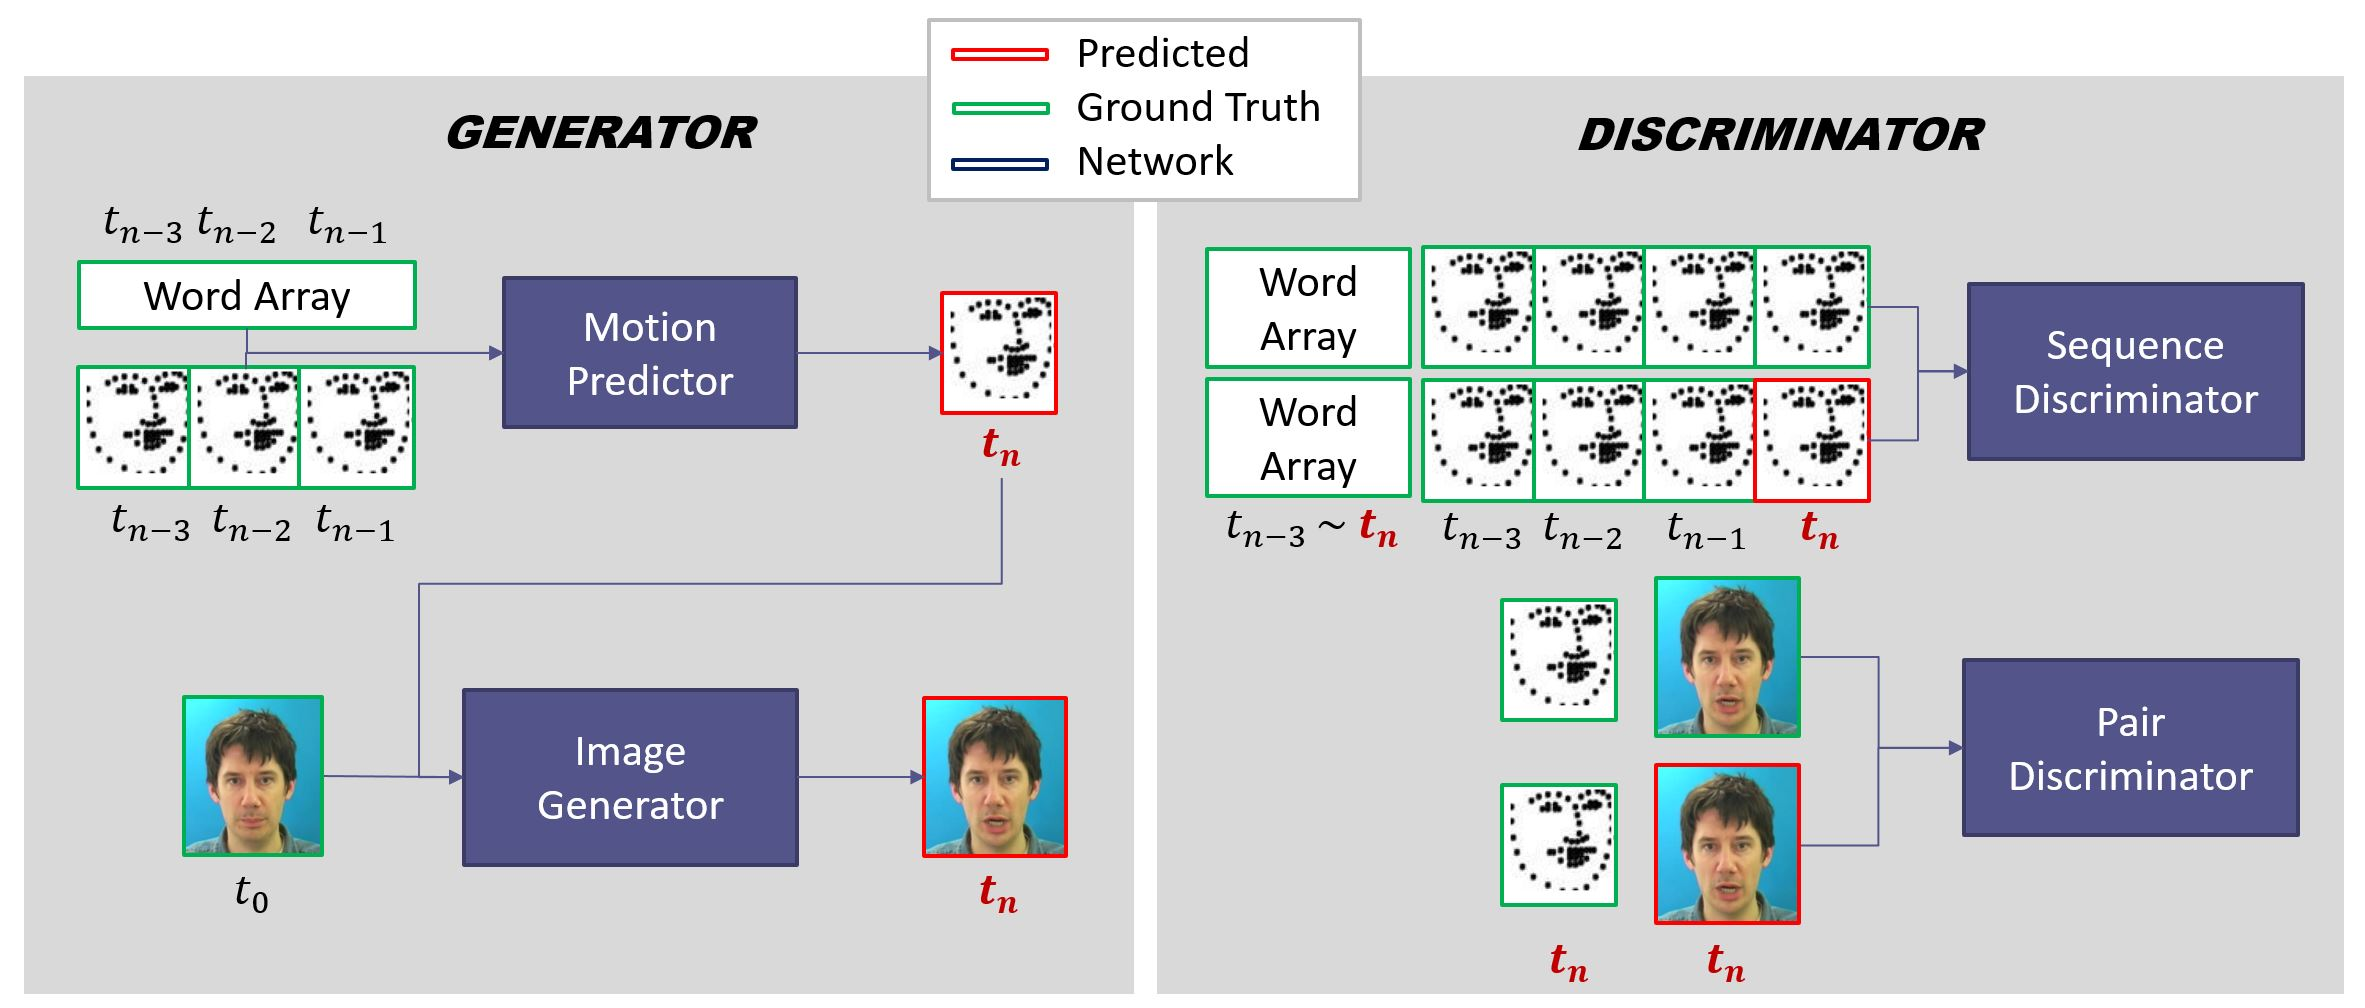
\includegraphics [scale=0.3] {images/network.JPG}
\end{center}
 \caption{The overall architecture of our network.  Generator consists of motion predictor, and image generator. Discriminator consists of sequence discriminator, and pair discriminator}
\label{fig:short}
\end{figure*}


\subsection{Two - Stage Generator}
The generator is comprised of motion predictor and the image generator. Motion predictor gets the condition and previous landmark positions and predicts the next landmark. Image generator gets this predicted landmark and initial photo to make a realistic image based on this landmark.

\subsubsection{Motion Predictor}
Motion predictor predicts the next motion based on the previous landmark information and condition. As we said above, the word information roles as a condition in this project. We first tiled the word information to make this have the same size as the landmark information have. Then we concatenated this word information with the initial landmark information. All the landmark information is represented as a table which represents x, and y value of all points. This concatenated information now feeds into the LSTM network.
\subsubsection{Image Generator}

Image generator uses an initial image and predicted landmarks. We used U-Net network to modify initial image based on the predicted landmarks. The landmark image and initial image is concatenated and passed through this network. U-Net network is a well-known network architecture which uses skip connections to reconstruct the image. For encoder and decoder part we all used the convolution layers and instance normalization layers. There are many ways for the decoder part to make the image size big. In this time, we used the transpose convolution as an upsampling.

When we trained this model we first trained the image generator with the ground truth landmark at time t to avoid errors from motion predictor. We thought the wrong output from motion predictor could hinder image generator and pair discriminator from converging. After we could sure that both motion predictor and image generator works quite well, we used the predicted landmarks to the image generator.
\subsection{Discriminator}
 There are two different types of a discriminator, sequence discriminator, and pair discriminator.
\subsubsection{Sequence Discriminator}
Sequence discriminator distinguishes between real sequence data and fake sequence data. Real sequence data is comprised of a ground truth initial frame and a current frame. Fake sequence data is comprised of a ground truth initial frame, previous frame, and fake current frame. Unlike other discriminators, this discriminator should get different size of the input at each time. To deal with this problem, we introduced the sequence discriminator which has the LSTM network as a basic structure. We used LSTM network which is said to be good at handling vanishing gradient problem through time.
This sequence discriminator also can be used as a word discriminator. All the concatenated data starts from the word information first. We expect that if we give a fake word at the first time and concatenate the ground truth sequence, the sequence discriminator should determine it as a false. In this paper, we are not using this modified form of sequence discriminator.
\subsubsection{Pair Discriminator}
Pair discriminator distinguishes between real pair data and fake pair data. Real pair data is concatenated by real landmark and real image. Fake pair data is concatenated by real landmark and predicted image from image generator. Real landmark is given as a condition to this network.
\section{Learning Prediction by Up-sampling}
The challenge in this predictor is due to the variety of trajectories of each landmark points. The trajectory could be different every time. This could be varied depends on how long that the word would be spoken, how loud or small the word would be spoken, and what word is said before. We thought the time length of each word mainly affects the difficulties of this problem.
To solve this variation of time problem, we are introducing $Learning$ $ prediction$ $by$ $upsampling$ method. This method assumes that the overall trajectory of each word is similar, and this trajectory is just scaled up with respect to the time length. The motion predictor would predict motion with the fixed number of time which should be larger than the maximum number of ground truth time length of each word. In other words, all the ground truth would be scaled up to some fixed length, and the motion predictor should predict the motion at every fixed length of time.
This approach is based on the Nyquist sampling theorem. If the sampling frequency is at least twice much higher than the original signal frequency, the sample would be sufficient to represent the original signal. The video sampling frequency should be at least twice much higher than the landmark analogous signal. Let's say there is a $N$ number of motion, $M_k$, in set $M = \big[\ M_k|M_1,M_2, ... , M_N\big]$. The video frequency of word $M_k$ can be represented like  $freq_{video}^{M_k}$, and original landmark analogous signal can be represented like $freq_{analog}^{M_k}$.This all can be represented like this using Nyquist sampling theorem.

\bigskip
\begin{center}
$freq_{video}^{M_k} \geq 2 \ast freq_{analog}^{M_k} $
\end{center}
\bigskip

In the same way, the prediction frequency,$freq_{pred}^{M_k}$, also should be at least twice much higher than the landmark analogous signal. This also can be represented like this.

\bigskip
\begin{center}
$freq_{pred}^{M_k} \geq 2 \ast freq_{analog}^{M_k} $
\end{center}
\bigskip

Combining this two equations, the prediction frequency is sufficient to be larger than the max video frequency. Then, prediction frequency would also be at least twice much higher than the landmark analogous signal.

\bigskip
\begin{center}
$freq_{pred}^{M_k} \geq MAX[freq_{analog}^{M_k}] $
\end{center}
\bigskip

This method can be represented like the left side of Figure 2.

\begin{figure*}
\begin{center}
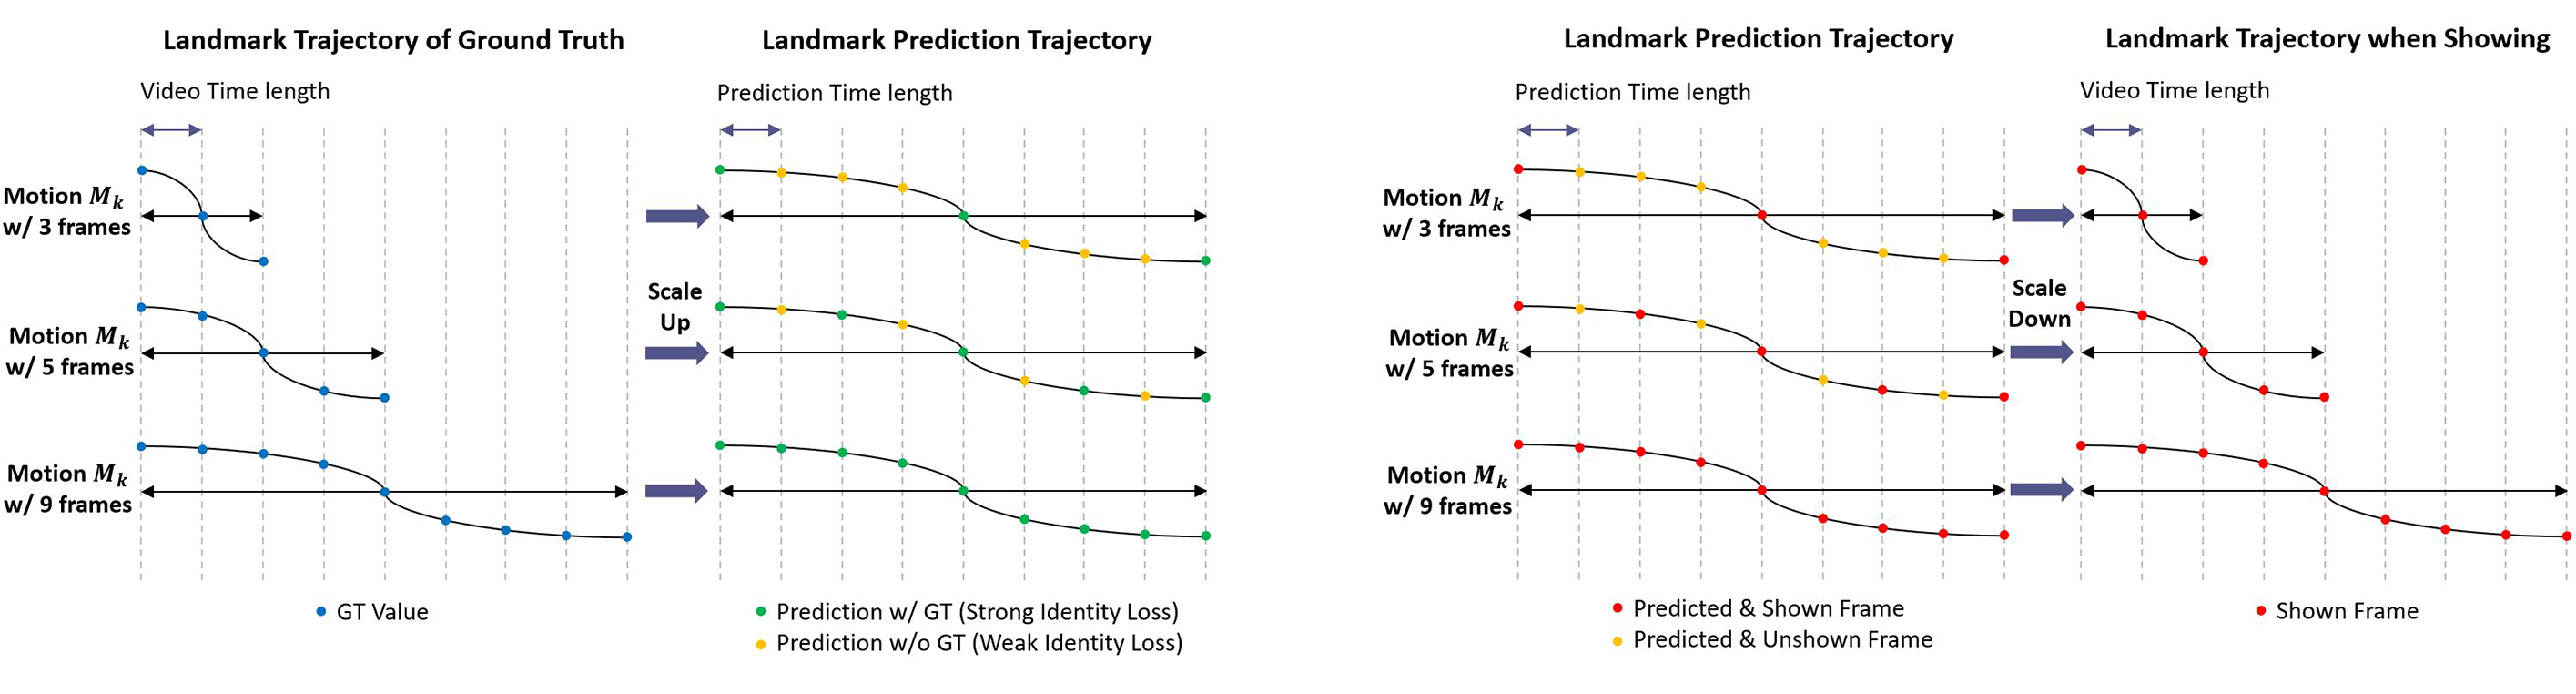
\includegraphics [scale=0.3] {images/upsample.JPG}
\end{center}
 \caption{$Left:$ Learning Prediction by Up-sampling. $Right:$ Prediction by Up-sampling. $Left:$ Same motion $M_k$ have the different number of frames. This GT value can be scaled up to specific fixed number of frames. $Right:$ Same motion $M_k$ is set to have the different number of frames. Sequence of shown frames at each row would be perceived to have motion like this.}
\label{fig:short}
\end{figure*}

Every different time length with the same motion is scaled up to the same amount of frame. The motion predictor predicts the motion every time and it is back-propagated every time. We introduced the ‘strong identity loss’ and ‘weak identity loss’. When there is a ground truth value, we adjust strong identity loss to minimize the value. If there is no ground truth value, we perform weak identity loss between predicted value and the next ground truth value. We used the L1 loss to minimize the distance between ground truth position and predicted position. And the weight is adjusted to achieve this objective.

With this method, the velocity of the motion also can be changed. This method can be verified when we test this model. Motion predictor predicts the fixed size of frames which is denser than the ground truth data. This means that if we change the amount of sampling ratio from motion predictor, the velocity of motion would be changed. If the sampling step size is big, the motion would be seemed to change rapidly. If the sampling step size is small, the motion would be seemed to change slowly. This method can be explained like the right side of Figure 2.



%------------------------------------------------------------------------
\section{Training}
 The GRID Corpus contains 33,0000 videos which when combined is over 2 million frames. Various length videos are difficult to batch, so we opted not to for the sake of development time as we had a limited amount of time to produce results. We used 32 of the speaker video sets for training and left 1 for testing to test a face not seen by the network before. Training one epoch on the entire dataset takes roughly 3 days. In the effort to reduce training time, we used only 30 of the 51 words. We still have yet to train the network on the entire dataset, due conducting several tests to find the best configuration.

%------------------------------------------------------------------------
\section{Experiments}

 After trying several network architectures, we found that a simpler 2-part approach with a motion prediction model and an image generation model using an initial frame and predicted landmarks was faster to train and produced better results. We performed a series of qualitative and quantitative tests. 
 
\subsection{UNet Image Generation}
 To test the image generator we performed a qualitative test to compare generated frames using ground truth landmarks with frames from ground truth videos. We are mostly interested in mouth movement, since the remaining parts of the face are expected to be static. We found the result is compelling. The mouth jitters which is caused by the landmark detection, but frame by frame it is difficult to tell which is image is fake. Teeth, tongue, and inner mouth is realistically generated. In motion the result can appear uncanny since the eyes and head pose remain perfectly stationary. We also did a qualitative study comparing 50 test videos with ground truth with an MSE score of \_.
 
\subsection{LSTM Motion Prediction}
 Producing realistic speech motion from words is a challenging problem. Fine motions must be learned for a human to distinguish the motions between words. Another challenge of learning speech motions are that the times to say a word vary between person and instance. We did a variety of qualitative and quantitative tests to identify where the model learned well and where it does not. 
 
 We conducted a qualitative experiment on how well our model can represent speech of a given word. Our goal is to produce plausible motions for a given word. Our current model is able to recreate up and down motions well, but the stretching the mouth corners outward (to produce sounds like 'e') and compressing the lips to form tight circles (for sounds like 'oo' or 'u') was not reproduced. We believe this is due to the smaller magnitude these motions produce when compared to the larger open and closing motions. The network learns there is a greater effect on minimizing the error by focusing on the up and down motions. We attempted to normalize the changes by applying a hyperbolic tangent function (Tanh) to the predicted and ground truth landmarks when computing the L1 loss. We were not able to fully train a network to asses how effective this was. While the initial inductions seem positive, the changes were too small and remain inconclusive. 
 
 Another qualitative test was to observe how well the model predicted face and landmarks when compared with ground truth. We found that the landmarks followed the open and close motions well for each word, though timings are imperfect. It is expected that the timings would not align well because only the landmark shape is personalize not how the word is uttered. 
 
 We quantitatively tested how well the predicted landmarks matched ground truth and compared the result with a video generated using ground truth landmarks. This is a challenging test due to the inability of our network to model person specific motions and timings. We also compared the generating a video between predicted landmarks and the initial landmark to see if we can produce a better result than doing nothing. We found it difficult to produce a result better than not moving the mouth. This is again likely due to the lack of word personalization and timing.
 
 To test predicting words being spoken over various time intervals, we had the network predict the same word for a different number of frames. In our example we use the word 'soon' and generated video consisting of 3, 7, and 10 frames. From the result it is clear that the network learned to predict words for different number of frames as intended.
 
\section{Conclusion}
We have shown it is possible to predict plausible mouth motions and generate photo-realistic video given words and an initial starting frame. We have also shown that our model can learn and predict the same motions for a given word over a different number of frames.  

{\small
\bibliographystyle{ieee}
\bibliography{egbib}
}



\end{document}




